\documentclass[12pt]{article}

\usepackage[margin=0.8 in]{geometry}
\usepackage{amsmath}
\usepackage{amssymb}
\usepackage{macros}
\usepackage{mathtools}
\usepackage{enumerate}
\usepackage{verbatim}
\usepackage{amsthm}

\title{}
%\content{}



\let \proj \undefined
\renewcommand{\tr}{ \mathrm{tr}}
\DeclareMathOperator{\SU}{SU}
\DeclareMathOperator{\proj}{proj}
\newcommand{\sS}{\mathscr{S}}
\DeclareMathOperator{\comp}{comp}
\newcommand{\A}{\mathcal{A}}
\renewcommand{\D}{\mathcal{D}}
\renewcommand{\e}{\epsilon}
\newcommand{\Are}{\A_{r,\e}}
\newcommand{\Kre}{K_{r,\e}}
\newcommand{\Dre}{\D_{r,\e}}
\newcommand{\rt}{\tilde{r}}
\newcommand{\et}{\tilde{\e}}
\newtheorem{definition}{Definition}
\newenvironment{solution}
  {\begin{proof}[Solution]}
  {\end{proof}}
\newtheorem{example}{Example}
\newtheorem{exercise}{Exercise}

\newcommand{\vr}{\mathbf{r}}
\newcommand{\vF}{\mathbf{F}}

\newtheorem{theorem}{Theorem}

\newcommand{\triple}{\iiint_E f(x,y,z) dV}

\begin{document}
\section*{15.7 Triple Integrals}
What to know:
\begin{enumerate}
\item Be able to set up a triple integral on a bounded domain of $\R^3$ in any of the 6 possible orders
\item Know the formula for volume and the one for mass from the applications.
\end{enumerate}

\subsection*{Triple integrals on box-shaped solids}
In the previous section we saw how we can use a double integral to compute the mass of a lamina (a 2-dimensional object). What if we'd like to find the mass of a solid in the shape of the box? If the box had the same density $\rho$ everywhere, then its mass would be $$Volume\times \rho.$$ Suppose it has variable density $\rho(x,y,z)$ and occupies the region 
$$B=\{(x,y,z):a\leq x\leq b, c\leq y\leq d,r\leq z\leq s\}$$
 we could split $[a,b]$, $[c,d]$, $[r,s]$ into $l, m, n$ subintervals respectively, to obtain small enough boxes of volume $\Delta V$ where the density is almost constant, calculate the mass of each box and add the resulting masses. That is, the volume would be approximately $$\sum_{i=1}^l\sum_{j=1}^m\sum_{k=1}^n\rho(x_i^*,y_j^*,z_k^*)\Delta V,$$ where $x_i^*$ is in the $i$th subinterval of $[a,b]$, $y_j^*$ in the $j$th subinterrval of $[c,d]$ and $z_k^*$ in the $k$th subinterval of $[r,s]$.  This expression really looks like a Riemann sum, with the approximation improving as we let $l, m , n \to \infty$, and indicates that it would make sense to define the integral of a function defined on a subset of $\R^3$, even though we don't have as a concrete of a geometric interpretation for it as we had for simple and double integrals. Thus we have:
 
 \begin{definition} If $f(x,y,z)$ is continuous and defined on a box $B$ as before, and we define $$\iiint_B f(x,y,z)dV:=\lim_{{l\to\infty}}\lim_{{m\to\infty}}\lim_{{n\to\infty}}\sum_{i=1}^l\sum_{j=1}^m\sum_{k=1}^n\rho(x_i^*,y_j^*,z_k^*)\Delta V.$$
 \end{definition}
 

Just as before, this definition is not particularly useful, but Fubini's theorem applies again:
\begin{theorem} If $f$ is continuous on $B=[a,b]\times[c,d]\x [r,s]$, then \begin{align*}
\iiint_B f(x,y,z)dV=&\int_a^b\int_c^d\int_r^sf(x,y,z)dzdydx\\
=&\int_a^b\int_r^s\int_c^df(x,y,z)dydzdx\\
=&\int_r^s\int_a^b\int_c^df(x,y,z)dydxdz\\
=&\dots \text{(3 more ways).}
\end{align*}
\end{theorem}


\textbf{Remark:} As the functions in this section are defined on subsets of $\R^3$ and take values in $\R$, visualizing them is difficult- we'd normally need 4 dimensions! Something we can do is try to understand their behavior through their level sets, i.e. sets of the form $$f^{-1}(c):=\{(x,y,z)\in\R^3:f(x,y,z)=c\},$$ which are generically 2 dimensional surfaces, assuming $f$ is sufficiently nice. (In Figure \ref{pic1} you can see a few level sets of the function $f(x,y,z)=x^2-y^2+z$). 

However, in integration, visualizing the function won't be of tremendous importance and we'll focus almost exclusively on visualizing the domain, which will be a solid in $\R^3$.



\begin{figure}
\centering
\parbox{5cm}{
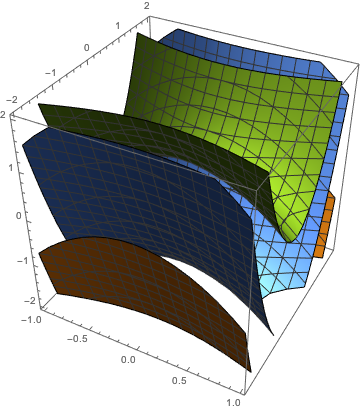
\includegraphics[width=5cm]{contour.png}
\caption{Some Level Sets}
\label{pic1}}
\qquad
\begin{minipage}{5cm}
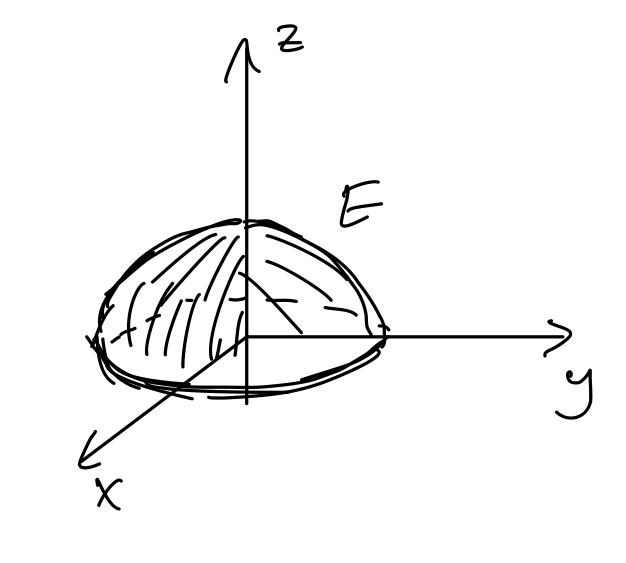
\includegraphics[width=5cm]{semisphere.jpeg}
\caption{From Example 1 and 2}
\label{fig10}
\end{minipage}
\end{figure}



\subsection*{Triple integrals on more general bounded solids}
We'll consider three main ways of describing domains and how triple integrals are written on them. Just like in double integrals, a domain might be able to be described in more than one ways or even in none of them. 

\begin{theorem}{(Bottom to Top integration)}
Let $E\subset \R^3$ be written in the form $$E=\{(x,y,z):(x,y)\in\D, u_1(x,y)\leq z\leq u_2(x,y)\}$$ and $f(x,y,z)$ be a continuous function on $E$. Then $$\iiint_E f(x,y,z)dV=\iint_D\big(\int_{u_1(x,y)}^{u_2(x,y)}f(x,y,z) dz\big) dA$$
\end{theorem}
\begin{figure}
\centering
\parbox{5cm}{
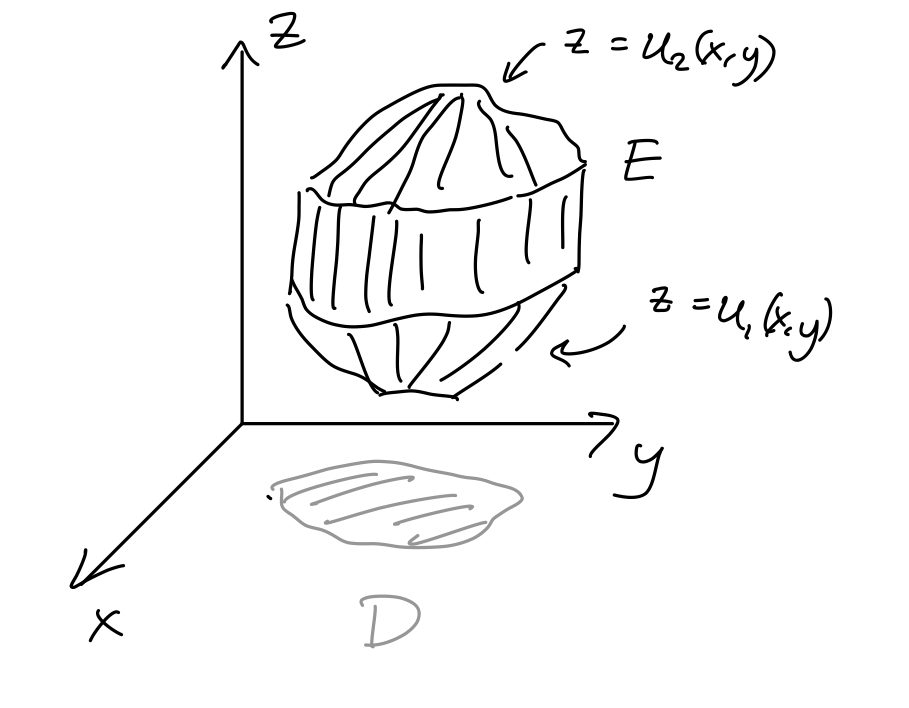
\includegraphics[width=5cm]{topbottom.jpg}
\caption{As in Theorem 2}
\label{fig5}}
\qquad
\begin{minipage}{5cm}
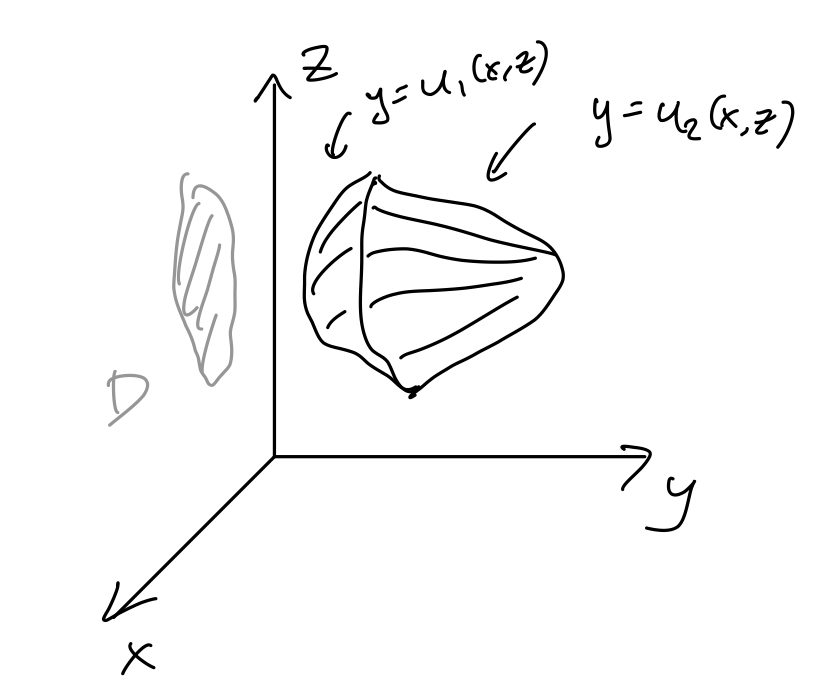
\includegraphics[width=5cm]{lefteright.jpg}
\caption{As in Theorem 4}
\label{fig6}
\end{minipage}
\end{figure}

\begin{theorem}{(Back to Front)}
Let $E\subset \R^3$ be written in the form $$E=\{(x,y,z):(y,z)\in\D, u_1(y,z)\leq x\leq u_2(y,z)\}$$ and $f(x,y,z)$ be a continuous function on $E$. Then $$\iiint_E f(x,y,z)dV=\iint_D\big(\int_{u_1(y,z)}^{u_2(y,z)}f(x,y,z) dx\big) dA$$
\end{theorem}

\begin{figure}
\centering
\parbox{5cm}{
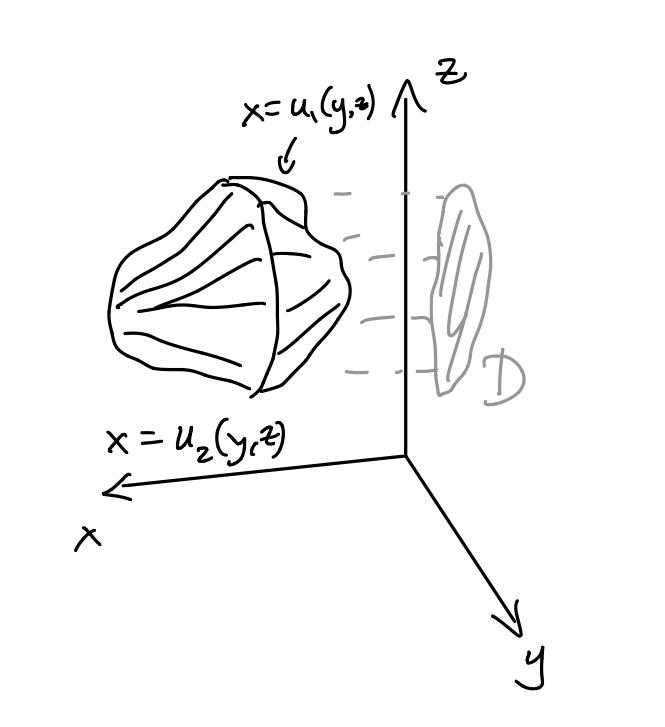
\includegraphics[width=5cm]{backfront.jpg}
\caption{As in Theorem 3}
\label{fig7}}
\qquad
\begin{minipage}{5cm}
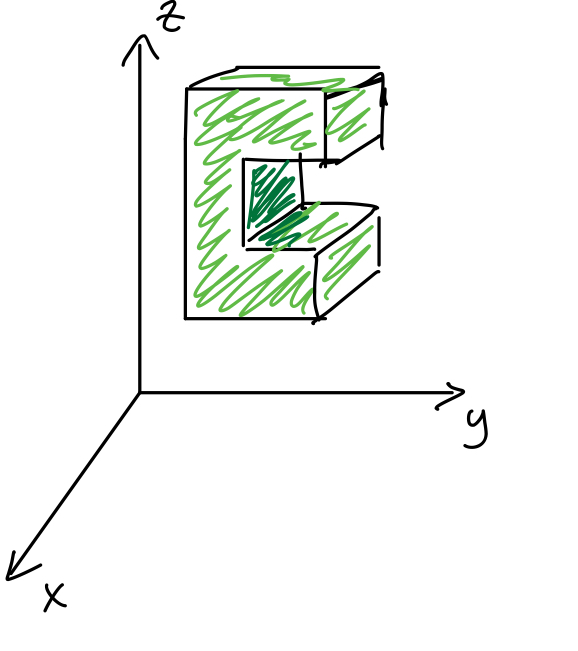
\includegraphics[width=5cm]{nottopbottom.jpg}
\caption{Not as in Theorem 2}
\label{fig8}
\end{minipage}
\end{figure}
\begin{theorem}{(Left to Right)}
Let $E\subset \R^3$ be written in the form $$E=\{(x,y,z):(y,z)\in\D, u_1(x,z)\leq y\leq u_2(x,z)\}$$ and $f(x,y,z)$ be a continuous function on $E$. Then $$\iiint_E f(x,y,z)dV=\iint_D\big(\int_{u_1(x,z)}^{u_2(x,z)}f(x,y,z) dy\big) dA$$
\end{theorem}

\textbf{Remarks:}
\begin{enumerate}
\item Each of the theorems above tells us that the calculation of the triple integral boils down to setting up a double integral. For instance, in Bottom to Top integration, if $\D=\{(x,y): a\leq x\leq b, g_1(x)\leq y\leq g_2(x)\}$ we have $$\iiint_E f(x,y,z)dV=\int_a^b\int_{g_1(x)}^{g_2{(x)}}\int_{u_1(x,y)}^{u_2(x,y)}f(x,y,z) dz dy dx$$
\item When setting up a triple integral, your final answer has to be a constant number. Therefore, the outermost integral needs to have constant bounds, the middle one may have functions of one variable as bounds and the innermost may have bounds that are functions of two variables.
\end{enumerate}

\subsection*{Some general guidelines for setting up triple integrals}
\begin{enumerate}
\item However hard it might be, try to draw a picture.
\item Write down all the equations corresponding to surfaces enclosing the domain. If you know which variable has to go into the innermost integral, solve for it in all equations (this might result in more equations, if, for example, this variable is squared).
\item If you're not told what order to set the integral up in, look for a variable that shows up twice in the equations and make it your innermost variable. Note that a squared variable might count as two!
\item Once you decide your innermost variable, say $z$, you're left with the task of finding the appropriate bounds for $x$ and $y$. To do this, you have to find the \textbf{projection} of your solid to the $xy$ plane. This can be done by intersecting the surfaces involving $z$ to eliminate it and end up with a number of equations describing curves in the $xy$ plane, i.e. involving only $x$ and $y$.
\item Use techniques from the previous lectures to find inequalities for the remaining variables to set up the double integral over them.
\item If you can easily find a specific point that has to live inside your solid, check if it satisfies all the inequalities you found. (If does, that's not guaranteeing that your setup is correct; however if it fails to satisfy even one of them, it means something is wrong).
\end{enumerate}

\textbf{Remark:} The process described in step 4 may generally result in redundant curves; you might find equations of $x, y$ that are not relevant  in setting up the integral. This is why drawing a picture is very useful. This will become clear in the examples.

\subsection*{Examples}
\begin{example} Set up the integral of $f(x,y,z)$, which is defined on the solid $E$ bounded by the surfaces $x^2+y^2+z^2=1$, $z=0$ and satisfying $z\geq 0$, in the order $dz dx dy$.
\end{example}
\begin{solution}
This is a bottom to top integration problem, so we need 2 functions $z=u_j(x,y),$ $j=1,2$. We have to use the lower bound $z=0$ and also solve for $z$ in $x^2+y^2+z^2=1$ to find $z=\sqrt{1-x^2-y^2}$. Therefore $$0\leq z\leq \sqrt{1-x^2-y^2}.$$

To find the bounds for $x, y$ we intersect the given surfaces $z=0$ and $x^2+y^2+z^2=1$ to find $x^2+y^2=1$, which tells us that $x, y$ live in the unit disk. Then as in the first week, we find $$-\sqrt{1-y^2}\leq x\leq \sqrt{1-y^2}$$ and $$-1\leq y\leq 1.$$

We can check that the point $(0,0,\frac{1}{2})$ that lies in $E$ satisfies all inequalities.

Finally $$\triple =\int_{-1}^1\int_{-\sqrt{1-y^2}}^{\sqrt{1-y^2}}\int_0^{\sqrt{1-x^2-y^2}} f(x,y,z) dz dx dy.$$
\end{solution}

\begin{example} Same as Example 1, in the order $dx dy dz$.
\end{example}
\begin{solution}
The 2 functions $x= u_i(y,z)$ are hidden inside $x^+y^2+z^2=1$. Solving for $x$, we find $x=\pm \sqrt{1-y^2-z^2}$ and therefore $$-\sqrt{1-y^2-z^2}\leq x\leq \sqrt{1-y^2-z^2}.$$

Then we look at the domain of $y, z$. Let's write down all of our surfaces:
\begin{align}
& x=-\sqrt{1-y^2-z^2}\label{eq2}\\
& x=\sqrt{1-y^2-z^2}\label{eq3}\\
& z=0. \label{eq4}
\end{align}
We see that \eqref{eq4} only involves $z$, so we don't need to do anything about it. However \eqref{eq2} and \eqref{eq3} both involve $x$, so we intersect them to eliminate it. We find $$y^2+z^2=1,$$ so as in week 1 we have $$-\sqrt{1-z^2}\leq y\leq \sqrt{1-z^2}$$
$$0\leq z\leq 1.$$

We check that the point $(0,0,\frac{1}{2})$ that lies in $E$ satisfies all inequalities.

Finally:
$$\triple =\int_0^1\int_{-\sqrt{1-z^2}}^{\sqrt{1-z^2}}\int_{-\sqrt{1-y^2-z^2}}^{\sqrt{1-y^2-z^2}}f(x,y,z)dx dydz.$$
\end{solution}


\begin{example}
Set up $\triple$ in the order $dz dx dy $, where $E$ is bounded below by $z=0$, bounded above by $z=2-x^2-y^2$ and is in the interior of the cylinder $x^2+y^2 = 1$.
\end{example}
\begin{figure}
\centering
\parbox{5cm}{
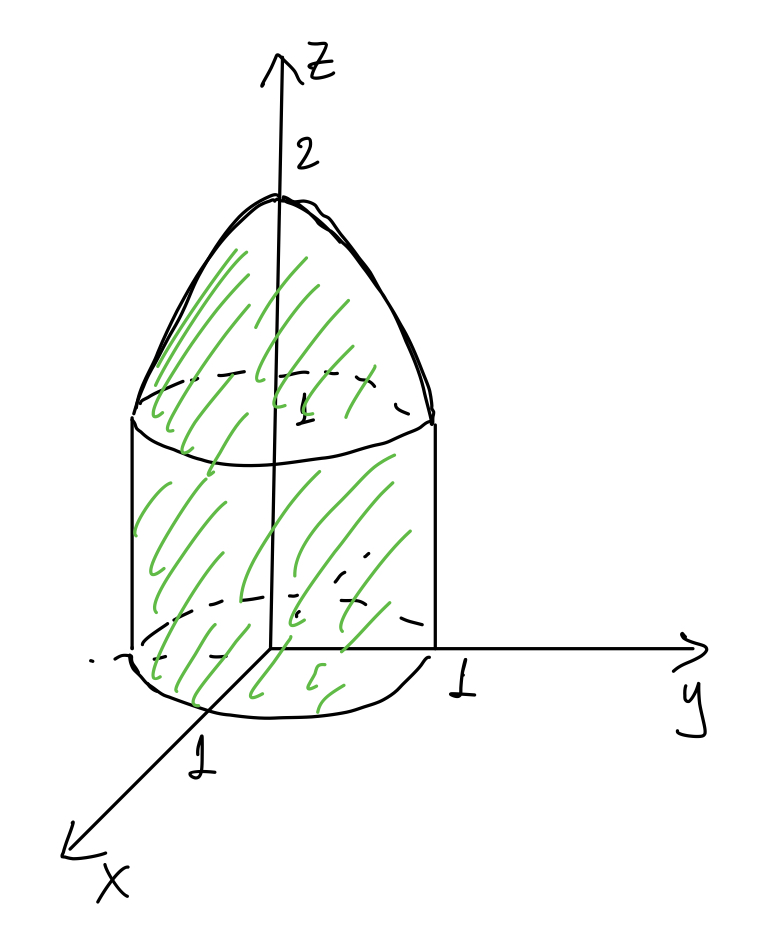
\includegraphics[width=5cm]{bullet1.jpeg}
\caption{Our solid}
\label{fig1}}
\qquad
\begin{minipage}{5cm}
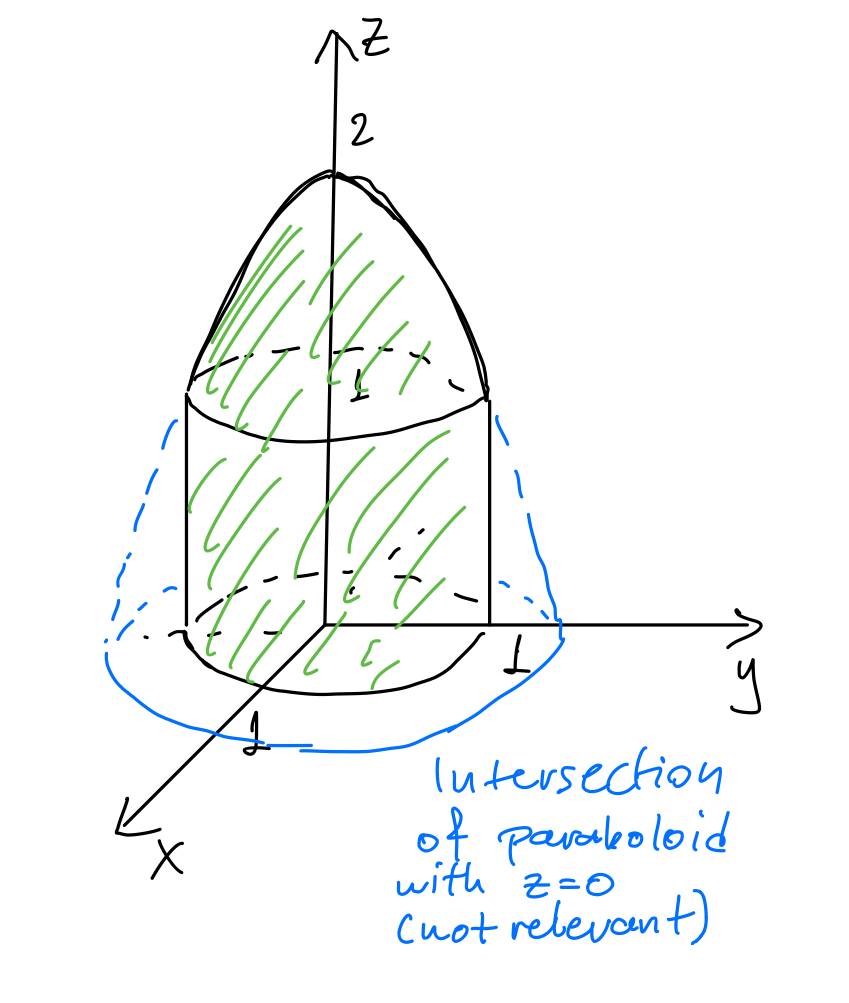
\includegraphics[width=5cm]{bullet2.jpeg}
\caption{The solid together with the intersection of the paraboloid and the $xy$ plane}
\label{fig2}
\end{minipage}
\end{figure}

We drw a picture as in Figure \ref{fig1} and list the equations of our boundary surfaces:
\begin{align}
& z=2-x^2-y^2\label{eq5}\\
& x^2+y^2 = 1 \label{eq6}\\
& z=0. \label{eq7}
\end{align}
This means $$0\leq z\leq 2-x^2-y^2.$$ We need to find the bounds for $x, y$. We see that \eqref{eq6} only involves $x$ and $y$ so we keep it. This is one of the cases when finding all relevant intersections leads to redundant equations and we need the picture to understand what's going on. If we intersect the equations involving $z$ we have:
$$ \eqref{eq5} \& \eqref{eq7}\implies x^2+y^2=2.$$
However, this curve is not relevant to our solid (look at the blue curve in Figure \ref{fig2}). Finally, we only have to use $$x^2+y^2=1, $$ and we find $$-\sqrt{1-y^2}\leq x\leq \sqrt{1-y^2}$$ and $$-1\leq y\leq 1.$$
Check that $(0,0,1)$ satisfies all inequalities.
So $$\triple =\int_{-1}^1\int_{-\sqrt{1-y^2}}^{\sqrt{1-y^2}}\int_0^{{2-x^2-y^2}} f(x,y,z) dz dx dy.$$

\begin{example}
Same as Example 3, in the order $dydxdz$.
\end{example}
\begin{solution}
Let's list all equations, solving for $y$, since this is the innermost integral.
\begin{align}
&y=\sqrt{1-x^2}\label{eq8}\\
&y=-\sqrt{1-x^2}\label{eq9}\\
&y=\sqrt{2-x^2-z}\label{eq10}\\
&y=-\sqrt{2-x^2-z}\label{eq11}\\
&z=0\label{eq12}
\end{align}
The integral can be set up as a left to right integral, but the two functions $y=u_i(x,z)$, $i=1,2$ don't have the same expression over their entire domain (we can see this because $y$ appears four times), so we can write it as a sum of integrals with an easier expression. Looking at a picture will be crucial in order to set this integral up correctly.

Let's try to understand the domain. We find the intersections that eliminate $y$, being careful about redundancy.
$$\eqref{eq8}\&\eqref{eq9}\implies x=\pm 1$$
$$\eqref{eq8}\&\eqref{eq10}\implies z=1$$
$$\eqref{eq8}\&\eqref{eq11}\implies z=1\text{ and }x=\pm 1 \text{ (that's only a point!)}$$
$$\eqref{eq9}\&\eqref{eq11}\implies z=1\text{ and }x=\pm 1 \text{ (again, only a point)}$$
$$\eqref{eq9}\&\eqref{eq11}\implies z=1$$
$$\eqref{eq10}\&\eqref{eq11}\implies z=2-x^2 \text{ or } x=\pm \sqrt{2-z}$$
We don't look at intersections with $\eqref{eq12}$ because it doesn't help eliminate $y$. Looking at the picture (Figure \ref{fig3}), we see what the the domains have to look like: We have $$D_1=\{(x,z): -1\leq x\leq 1, 0\leq z \leq 1\}$$ and $$D_2=\{(x,z): -\sqrt{2-z}\leq x\leq \sqrt{2-z}, 1\leq z \leq 2\}$$
\begin{figure}
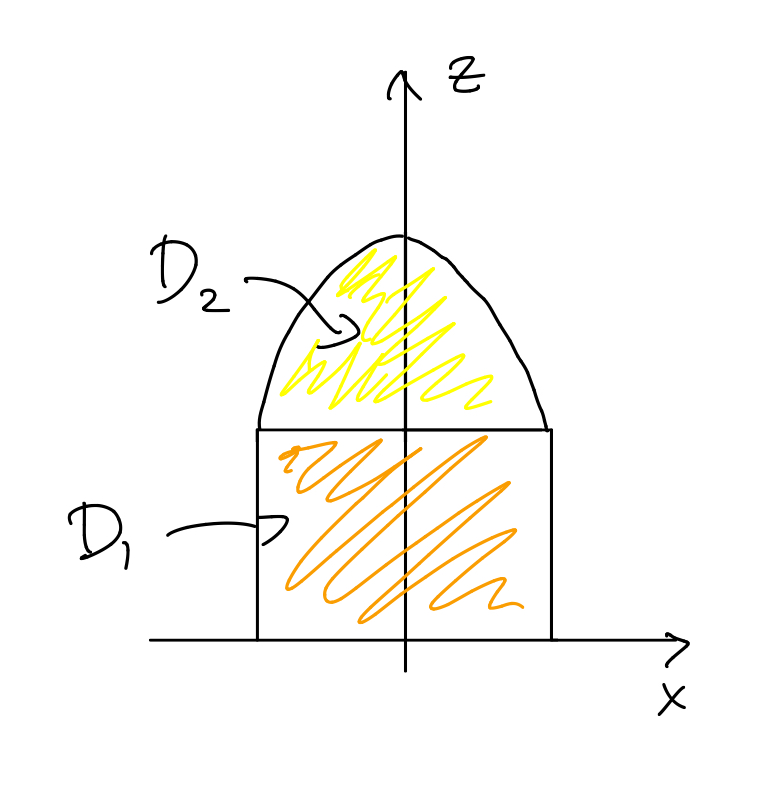
\includegraphics[width=5 cm]{projection1.jpeg}
\caption{The projection on the $xz$ plane}
\label{fig3}
\end{figure}
Over $D_1$ we have $$-\sqrt{1-x^2}\leq y\leq \sqrt{1-x^2}$$ and over $D_2$ we have $$-\sqrt{2-x^2-z}\leq y \leq \sqrt{2-x^2-z}.$$

Finally $$\triple=\int_0^1\int_{-1}^1\int_{-\sqrt{1-x^2}}^{\sqrt{1-x^2}}f(x,y,z)dydxdz+\int_1^2\int_{-\sqrt{2-z}}^{\sqrt{2-z}}\int_{-\sqrt{2-x^2-z}}^{\sqrt{2-x^2-z}}f(x,y,z)dydxdz.$$

\end{solution}

\subsection*{Applications}
\begin{enumerate} 
\item \textbf{Volume:} In a way analogous to double integrals, the Volume of a solid is given by $$V(E)=\iiint_V 1 dV$$
\item \textbf{Center of Mass: } Analogously to double integrals, the center of mass of a solid is $$(\bar{x},\bar{y},\bar{z})=(\frac{M_{yz}}{M},\frac{M_{xz}}{M},\frac{M_{xy}}{M}),$$ where $$M=\iint_E \rho(x,y,z)dV$$ is its \textbf{mass}, 
$$M_{yz}=\iint_E x\rho(x,y,z)dV$$ is the \textbf{moment about the $yz$ plane},
$$M_{xz}=\iint_E y\rho(x,y,z)dV$$ is the \textbf{moment about the $xz$ plane} and
$$M_{xy}=\iint_E z\rho(x,y,z)dV$$ is the \textbf{moment about the $xy$ plane} and $\rho$ is the density of the solid.
\end{enumerate}
\end{document}

